% fig_6_2_future_roadmap -- TikZ source of thesis Figure 20 (fig:future_roadmap).
% Every label is taken from the text of thesis Chapters 4 and 6.
% Limitation tags and short labels are the same as in Fig. 19 (fig_5_1_contributions_overview).
% Sizes (KTU thesis guide, section 5.1: figure text >= 10 pt): all text at 10 pt (normalsize of the 10 pt
% standalone), column headers 12 pt bold; each row's three boxes take the height of its tallest text, so
% nothing is cramped.
% Natural width 15.44 cm: include at width=\textwidth (15.5 cm text block), scale ~1.
\documentclass[border=1pt]{standalone}
\usepackage[T1]{fontenc}
\usepackage{newtxtext,newtxmath}
\usepackage{amsmath}
\usepackage{tikz}
\usetikzlibrary{arrows.meta,calc,backgrounds}

% Print-safe pale fills (luminance ~91-94%), dark borders/tags, black text.
\definecolor{lFill}{RGB}{251,239,216}\definecolor{lEdge}{RGB}{130,85,15}   % limitation (as Fig. 19)
\definecolor{sFill}{RGB}{239,233,246}\definecolor{sEdge}{RGB}{100,70,135}   % remedy strand (as Fig. 19)
\definecolor{dFill}{RGB}{226,240,237}\definecolor{dEdge}{RGB}{40,105,95}    % deliverable
\definecolor{nFill}{RGB}{238,238,238}\definecolor{nEdge}{RGB}{110,110,110}  % open challenge (grey)
\definecolor{arrow}{RGB}{70,70,70}

% inline tags: filled for L1-L8, outlined for the LoRA-UNI2-h extension (not one of L1-L8)
\newcommand{\Ltag}[1]{{\setlength{\fboxsep}{1.3pt}\colorbox{lEdge}{\makebox[1.45em]{\textcolor{white}{\bfseries #1}}}}}
\newcommand{\Gtag}[1]{{\setlength{\fboxsep}{1.3pt}\colorbox{nEdge}{\makebox[1.45em]{\textcolor{white}{\bfseries #1}}}}}
\newcommand{\Otag}[1]{{\setlength{\fboxsep}{1.0pt}\setlength{\fboxrule}{0.5pt}\fcolorbox{lEdge}{white}{\textcolor{lEdge!80!black}{\bfseries #1}}}}

% column geometry (cm): limitation 0-4.95, remedy 5.35-11.20, deliverable 11.60-15.35
\newcommand{\xL}{2.475}\newcommand{\xR}{8.275}\newcommand{\xD}{13.475}
% \roadrow{box style}{arrow style}{row name}{limitation}{remedy}{deliverable}
% text nodes are placed at the current row top (rt); the three boxes are drawn behind them down to the
% lowest text bottom of the row; the arrows sit at the row's vertical middle; rt moves below the row.
\newcommand{\roadrow}[6]{%
  \node[limt, anchor=north] (#3L) at (xLc |- rt) {#4};
  \node[remt, anchor=north] (#3R) at (xRc |- rt) {#5};
  \node[delt, anchor=north] (#3D) at (xDc |- rt) {#6};
  \path let \p1=(#3L.south), \p2=(#3R.south), \p3=(#3D.south) in coordinate (#3b) at (0,{min(\y1,\y2,\y3)});
  \begin{scope}[on background layer]
    \filldraw[box, fill=lFill, draw=lEdge, #1] (xLa |- rt) rectangle (xLb |- #3b);
    \filldraw[box, fill=sFill, draw=sEdge, #1] (xRa |- rt) rectangle (xRb |- #3b);
    \filldraw[box, fill=dFill, draw=dEdge, #1] (xDa |- rt) rectangle (xDb |- #3b);
  \end{scope}
  \coordinate (#3m) at ($(rt)!0.5!(#3b)$);
  \draw[#2] (xLb |- #3m) -- (xRa |- #3m);
  \draw[#2] (xRb |- #3m) -- (xDa |- #3m);
  \coordinate (rt) at ($(#3b)+(0,-0.40)$);}

\begin{document}
\hyphenpenalty=10000 \exhyphenpenalty=10000
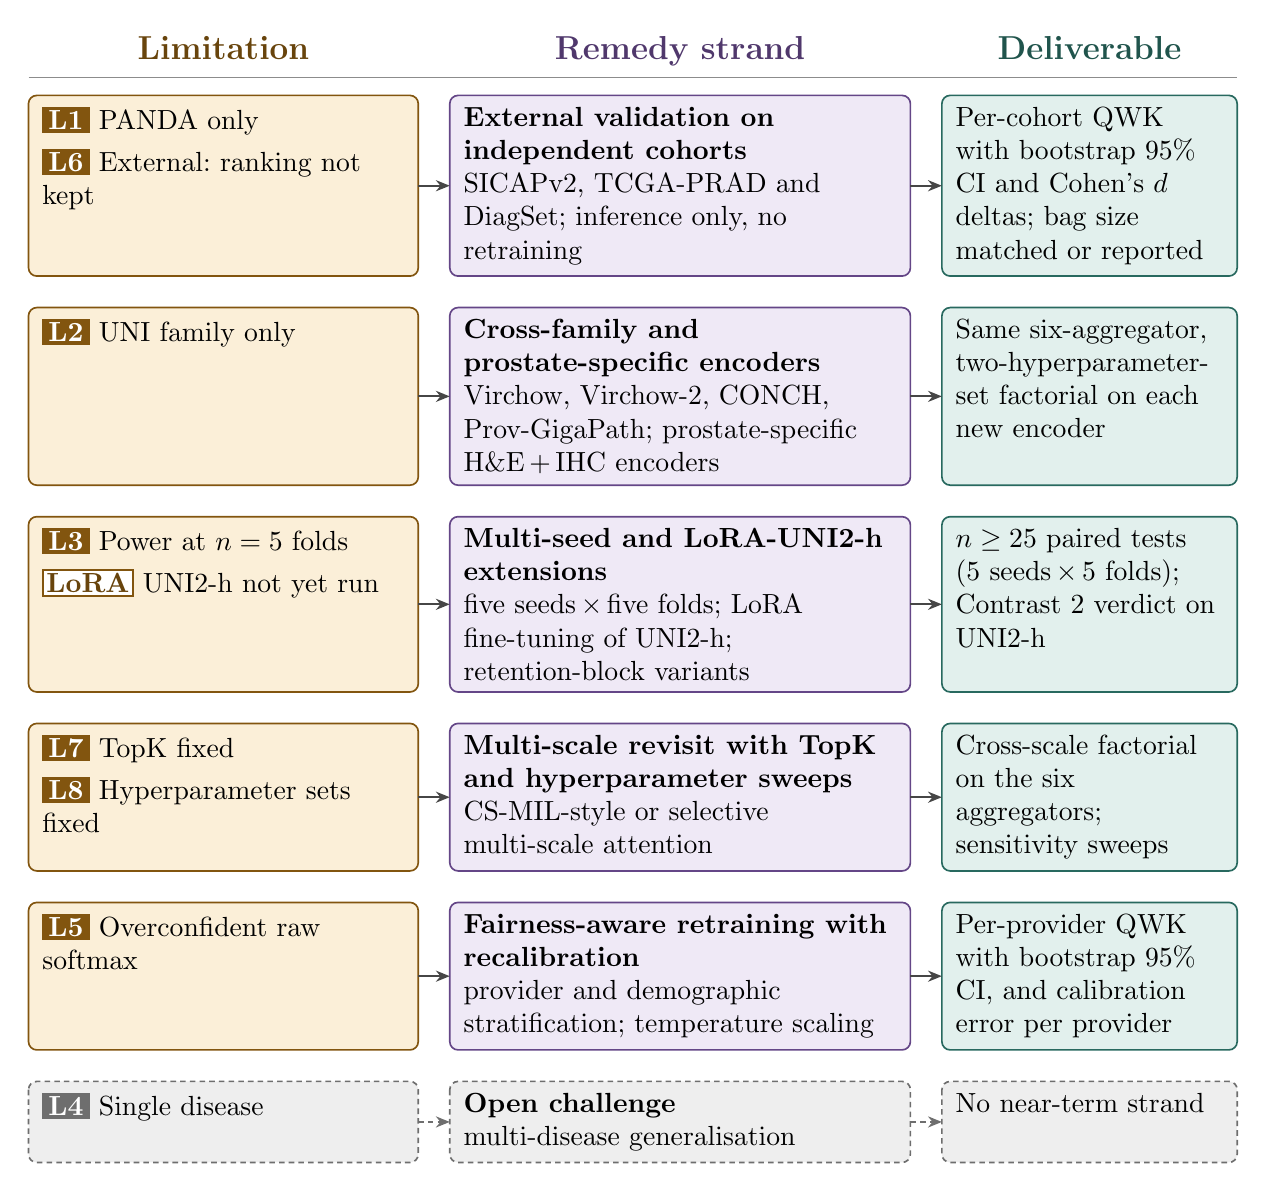
\begin{tikzpicture}[x=1cm, y=1cm, font=\normalsize,
    box/.style={rounded corners=3pt, line width=0.6pt},
    txt/.style={align=flush left, inner xsep=5pt, inner ysep=4pt},
    limt/.style={txt, minimum width=4.95cm, text width=4.95cm-10pt},
    remt/.style={txt, minimum width=5.85cm, text width=5.85cm-10pt},
    delt/.style={txt, minimum width=3.75cm, text width=3.75cm-10pt},
    grey/.style={fill=nFill, draw=nEdge, dash pattern=on 2pt off 1.5pt},
    arr/.style={-{Stealth[length=5pt, width=4pt]}, line width=0.8pt, draw=arrow},
    narr/.style={arr, draw=nEdge, dash pattern=on 2pt off 1.5pt},
    hdr/.style={font=\large\bfseries, anchor=base}]
  \coordinate (xLa) at (0,0);     \coordinate (xLb) at (4.95,0);
  \coordinate (xRa) at (5.35,0);  \coordinate (xRb) at (11.20,0);
  \coordinate (xDa) at (11.60,0); \coordinate (xDb) at (15.35,0);
  \coordinate (xLc) at (\xL,0);   \coordinate (xRc) at (\xR,0);   \coordinate (xDc) at (\xD,0);

  % ---- headers (exactly: Limitation / Remedy strand / Deliverable) ----
  \node[hdr, text=lEdge!80!black] at (\xL,-0.40) {Limitation};
  \node[hdr, text=sEdge!80!black] at (\xR,-0.40) {Remedy strand};
  \node[hdr, text=dEdge!80!black] at (\xD,-0.40) {Deliverable};
  \draw[line width=0.4pt, draw=black!45] (0,-0.62) -- (15.35,-0.62);
  \coordinate (rt) at (0,-0.85);

  % ---- row 1: external validation (L1, L6) ----
  \roadrow{}{arr}{ra}
    {\Ltag{L1}~PANDA only\\[3pt]\Ltag{L6}~External:\ ranking not kept}
    {\textbf{External validation on independent cohorts}\\ SICAPv2, TCGA-PRAD and DiagSet; inference only, no retraining}
    {Per-cohort QWK with bootstrap 95\% CI and Cohen's $d$ deltas; bag size matched or reported}
  % ---- row 2: cross-family and prostate-specific encoders (L2) ----
  \roadrow{}{arr}{rb}
    {\Ltag{L2}~UNI family only}
    {\textbf{Cross-family and prostate-specific encoders}\\ Virchow, Virchow-2, CONCH, Prov-GigaPath; prostate-specific H\&E\,+\,IHC encoders}
    {Same six-aggregator, two-hyperparameter-set factorial on each new encoder}
  % ---- row 3: multi-seed and LoRA-UNI2-h extensions (L3 + LoRA-UNI2-h) ----
  \roadrow{}{arr}{rc}
    {\Ltag{L3}~Power at $n = 5$ folds\\[3pt]\Otag{LoRA}~UNI2-h not yet run}
    {\textbf{Multi-seed and LoRA-UNI2-h extensions}\\ five seeds\,$\times$\,five folds; LoRA fine-tuning of UNI2-h; retention-block variants}
    {$n \geq 25$ paired tests (5~seeds\,$\times$\,5~folds); Contrast~2 verdict on UNI2-h}
  % ---- row 4: multi-scale revisit (L7, L8) ----
  \roadrow{}{arr}{rd}
    {\Ltag{L7}~TopK fixed\\[3pt]\Ltag{L8}~Hyperparameter sets fixed}
    {\textbf{Multi-scale revisit with TopK and hyperparameter sweeps}\\ CS-MIL-style or selective multi-scale attention}
    {Cross-scale factorial on the six aggregators; sensitivity sweeps}
  % ---- row 5: fairness-aware retraining (L5) ----
  \roadrow{}{arr}{re}
    {\Ltag{L5}~Overconfident raw softmax}
    {\textbf{Fairness-aware retraining with recalibration}\\ provider and demographic stratification; temperature scaling}
    {Per-provider QWK with bootstrap 95\% CI, and calibration error per provider}
  % ---- row 6: L4, open challenge (grey) ----
  \roadrow{grey}{narr}{rf}
    {\Gtag{L4}~Single disease}
    {\textbf{Open challenge}\\ multi-disease generalisation}
    {No near-term strand}
\end{tikzpicture}
\end{document}
